\begin{abstract}
We study whether nonlinear machine-learning models can improve next-month
cross-sectional U.S. equity return forecasts, and whether those forecasts
survive a disciplined long-short implementation after transaction costs. The
empirical design uses only course-provided Monthly CRSP and Compustat-style
data, with a final audited expanding-window walk-forward protocol
that evaluates annual out-of-sample test folds from 2017 through 2024. The
main specification combines return features with an audited flow-only
Compustat block and maps monthly predictions into equal-weight top-minus-bottom
decile portfolios. The strongest result is the flow-Compustat MLP,
which delivers net Sharpe 2.03 at 10 bps, annualized net return 21.4\%, a
rank-IC HAC $t$-statistic of 6.36, and breakeven costs near 90 bps. The
strategy strongly outperforms same-protocol reversal and z-score reversal
benchmarks. Momentum remains the strongest classical comparator; the ML
strategies are economically stronger, but mean-difference tests versus
momentum are not strongly significant. Performance is higher in bear and
high-volatility states, yet direct regime-feature ablations do not improve the
strong flow-Compustat models. The central limitation is that the provided
Monthly CRSP extract omits \code{prc}, \code{shrout}, \code{shrcd}, and
\code{exchcd}, so the report supports a credible flat-cost academic result
rather than a full tradability proof.
\end{abstract}

\section{Introduction}

Short-term reversal is one of the oldest cross-sectional return patterns in
equity markets, but it is not obviously stable enough to trade in raw form.
Naive reversal portfolios are high-turnover, sensitive to market conditions,
and often strongest in parts of the universe where implementation is hardest.
The more relevant question for a machine-learning project is therefore not
whether reversal exists mechanically, but whether conditional expected returns
can be estimated well enough to rank stocks more profitably than simple fixed
rules.

This project treats machine learning as a cross-sectional forecasting and
ranking problem. Each month, the model observes lagged stock-level return
signals, optionally augments them with audited flow-only firm
characteristics, and predicts next-month returns. Those forecasts are then
converted into market-neutral long-short portfolios and evaluated under a
shared backtest engine with flat transaction costs. The resulting claim is
economic rather than purely statistical: ML is useful only if it improves
out-of-sample ranking and retains performance after realistic turnover
penalties.

The report makes five contributions. First, it uses a final audited
expanding-window protocol designed to prevent leakage and align all model
comparisons. Second, it
compares nonlinear models against both linear benchmarks and same-protocol
classical reversal/momentum strategies. Third, it studies cost sensitivity
through turnover and breakeven transaction-cost analysis. Fourth, it treats
regime dependence both as an evaluation dimension and as a direct feature
ablation question. Fifth, it states clearly what cannot be claimed under the
assignment's no-external-data rule.

\section{Data and Prediction Problem}

The empirical target comes from Monthly CRSP. For stock $i$ at month $t$, the
main label is next-month return,
\[
R_{i,t+1} = \texttt{target\_ret\_fwd\_1m}.
\]
The report focuses on this raw return target. A supplementary
robustness exercise replaces it with market-adjusted next-month return,
\code{target\_excess\_ret\_fwd\_1m}, but that does not replace the main
result.

Predictors come from two admissible sources within the course data. The first
is a return-feature block constructed from lagged CRSP information. The second
is an audited flow-only Compustat block merged point-in-time with
conservative availability rules. No external datasets are used. The sample
spans 1984-01-31 through 2024-11-30, while the out-of-sample test
window covers 2017-2024. The walk-forward design keeps the training start
fixed at 1985-01-31 and rolls forward by calendar test year.

\begin{table}[t]
\centering
\small
\begin{tabular}{@{}lr@{}}
\toprule
Statistic & Value \\
\midrule
Sample period & 1984-01-31 to 2024-11-30 \\
Stock-months & 3,646,731 \\
Unique stocks & 33,884 \\
Average stocks per month & 7,427 \\
Baseline return features & 15 \\
Main target & \code{target\_ret\_fwd\_1m} \\
Target mean & 0.85\% \\
Target volatility & 18.39\% \\
\bottomrule
\end{tabular}
\caption{Sample overview used in the final pipeline.
\source{\code{table\_data\_summary.csv} in \code{report/tables/}}}
\label{tab:data-summary}
\end{table}

Table~\ref{tab:data-summary} summarizes the sample. Two additional facts from
the feature audit matter for interpretation. First, the Compustat
integration reports zero point-in-time violations. Second, roughly 66.8\% of
panel rows have at least one flow-only Compustat field available, which is
enough to matter economically without redefining the whole sample around a
small subset of firms.

The largest scope constraint is a missing-data one rather than a modeling one.
The provided Monthly CRSP extract lacks \code{prc}, \code{shrout},
\code{shrcd}, and \code{exchcd}. Under the assignment's no-external-data rule,
that means the project cannot implement true price, share-code, exchange,
microcap, or liquidity screens. The correct interpretation is therefore
flat-cost robustness on the provided universe, not a full executable
tradability study.

\section{Features, Models, and Validation Design}

The baseline feature family, \code{return\_only}, is built entirely from
lagged CRSP returns. It includes recent returns, intermediate-horizon
momentum, trailing volatility, drawdown, market beta, idiosyncratic
volatility, and cross-sectional rank transforms. These variables are designed
to let the model learn where reversal is strong, weak, or overturned by other
return dynamics.

The main feature family, \code{flow\_compustat}, augments those return signals
with audited flow-only firm characteristics such as sales, cost of goods sold,
capital expenditure, research and development, SG\&A, margins, growth rates,
and intensity ratios. These are the final Compustat inputs because the
reviewed extract supports them with defensible point-in-time timing. Balance
sheet style ratios are not part of the active pipeline because they are not
reliably available in the provided schema.

The model comparison has three layers. The classical baselines are reversal,
z-score reversal, momentum, and reversal plus momentum. The historical linear
benchmarks are Ridge and Elastic Net. The nonlinear models are XGBoost and a
compact MLP trained with regularization and early stopping. The report centers
on the final hierarchy in which the main comparison set is
return-only XGBoost, return-only MLP, flow-Compustat XGBoost, and
flow-Compustat MLP.

Validation is strict. For each annual test fold $Y \in \{2017,\ldots,2024\}$,
training uses data from 1985-01-31 through $Y-6$, validation uses the next
five years $Y-5$ through $Y-1$, and the held-out calendar year $Y$ is the
test period. Hyperparameters are selected on validation data only. Targets are
shifted forward by one month, predictors are available at time $t$, and only
out-of-sample predictions enter the backtest. The detailed ML-only
comparison is recorded in \code{table\_walkforward\_model\_summary.csv}; it
shows that the linear models remain materially weaker than the nonlinear
specifications.

Preprocessing is fold-specific as well. Continuous predictors are winsorized
and rank-normalized using training information only, missing values are
imputed without using future observations, and missingness indicators are
retained when they add information. That discipline matters because the
Compustat block is informative partly through selective availability, and any
full-sample transformation would contaminate the walk-forward evaluation.

\section{Portfolio Construction and Transaction Costs}

The forecasting problem is evaluated as a ranking problem. Each month, model
scores are converted into cross-sectional ranks, and the strategy goes long
the top 10\% of names and short the bottom 10\%. Long and short sleeves are
equal-weighted, so gross leverage is 2 and net market exposure is
approximately zero by construction. Alternative 5\% and 20\% cutoffs are part
of the robustness suite, but the 10\% specification is the headline
reporting standard.

Transaction costs are modeled as a flat basis-point charge on turnover:
\[
R^{\text{net}}_{p,t+1}
=
R^{\text{gross}}_{p,t+1}
- c \times \text{turnover}_{t},
\]
where $c$ is the round-trip cost expressed in decimal form. The main table
uses $10$ bps, and robustness considers a wider grid from zero to 100 bps.
This cost model is intentionally simple. It is useful for comparing signals on
a common footing, but it does not substitute for a full liquidity-aware
execution model, especially given the missing tradability fields described
above.

The shared portfolio engine also sharpens interpretation. Every strategy is
judged under the same decile cutoff, equal-weighting rule, rebalance
frequency, and cost convention, so performance differences can be attributed
primarily to signal quality rather than to inconsistent construction choices.
That is especially important when comparing ML models with classical baselines,
because raw forecast scale matters less than cross-sectional ranking power.

\section{Results}

Table~\ref{tab:hierarchy} is the central economic ranking of
strategies. It combines the detailed walk-forward model table with the
same-protocol classical baselines and focuses on the strategies that define
the report's main story.

\begin{table*}[t]
\centering
\scriptsize
\setlength{\tabcolsep}{4.5pt}
\begin{tabular*}{\textwidth}{@{\extracolsep{\fill}} llrrrrrr@{}}
\toprule
Strategy & Role & Net SR & Gross SR & Net ann. & Turnover & Breakeven & Rank-IC $t$ \\
\midrule
Flow-Compustat $\times$ MLP & Main model & 2.028 & 2.281 & 21.4\% & 2.21 & 90.5 & 6.36 \\
Flow-Compustat $\times$ XGBoost & ML comparison & 1.770 & 1.987 & 21.3\% & 2.18 & 91.4 & 3.54 \\
Return-only $\times$ XGBoost & ML comparison & 1.313 & 1.531 & 18.0\% & 2.50 & 70.1 & 2.09 \\
Return-only $\times$ MLP & ML comparison & 1.192 & 1.512 & 12.3\% & 2.76 & 47.2 & 4.04 \\
Momentum & Strongest classical benchmark & 0.636 & 0.683 & 15.0\% & 0.92 & 145.6 & 3.34 \\
Reversal plus momentum & Combined benchmark & 0.491 & 0.662 & 8.2\% & 2.40 & 38.6 & 2.74 \\
Reversal & Classical benchmark & 0.062 & 0.224 & 1.4\% & 3.13 & 13.9 & -0.12 \\
Z-score reversal & Classical benchmark & 0.062 & 0.224 & 1.4\% & 3.13 & 13.9 & -0.12 \\
\bottomrule
\end{tabular*}
\caption{Final model hierarchy under the final audited expanding-window
walk-forward protocol. \source{\code{table\_final\_model\_hierarchy.csv}
in \code{report/tables/}}}
\label{tab:hierarchy}
\end{table*}

Four conclusions stand out. First, nonlinear models dominate the linear
benchmarks and the raw reversal rules. The strongest specification is
the flow-Compustat MLP, which combines net Sharpe 2.03 with gross Sharpe 2.28
and annualized net return 21.4\% at 10 bps. Second, audited firm-level flow
features materially improve the nonlinear models. Relative to the return-only
MLP, the flow-Compustat MLP gains roughly 84 basis points of monthly mean
spread, lifts net Sharpe from 1.19 to 2.03, and raises breakeven costs from
47 to 90 bps. The same direction holds for XGBoost, though less strongly.

\begin{table*}[t]
\centering
\scriptsize
\setlength{\tabcolsep}{4.5pt}
\begin{tabular*}{\textwidth}{@{\extracolsep{\fill}} llrrrrrr@{}}
\toprule
Feature set & Model & Gross SR & Net SR & Net ann. & Turnover & Breakeven & Rank-IC $t$ \\
\midrule
Flow-Compustat & MLP & 2.281 & 2.028 & 21.4\% & 2.21 & 90.5 & 6.36 \\
Flow-Compustat & XGBoost & 1.987 & 1.770 & 21.3\% & 2.18 & 91.4 & 3.54 \\
Return-only & XGBoost & 1.531 & 1.313 & 18.0\% & 2.50 & 70.1 & 2.09 \\
Return-only & MLP & 1.512 & 1.192 & 12.3\% & 2.76 & 47.2 & 4.04 \\
Flow-Compustat & Elastic Net & 0.438 & 0.237 & 3.2\% & 2.25 & 21.8 & 0.99 \\
Flow-Compustat & Ridge & 0.234 & -0.005 & -0.1\% & 2.08 & 9.8 & 1.36 \\
Return-only & Elastic Net & 0.088 & -0.109 & -1.8\% & 2.66 & 4.5 & 0.69 \\
Return-only & Ridge & -0.162 & -0.284 & -6.4\% & 2.29 & -13.3 & -0.72 \\
\bottomrule
\end{tabular*}
\caption{Detailed ML-only walk-forward comparison.
\source{\code{table\_walkforward\_model\_summary.csv} in \code{report/tables/}}}
\label{tab:ml-detail}
\end{table*}

Table~\ref{tab:ml-detail} makes the linear-versus-nonlinear gap explicit. Even
after the audited flow-only Compustat extension, the linear models are
economically weak, with flow-Compustat Elastic Net at net Sharpe 0.24 and
flow-Compustat Ridge effectively zero after costs. The return-only linear
models are outright negative net at 10 bps. That matters because it rules out
a weaker interpretation in which any modest predictive fit would survive the
portfolio step; the gain is concentrated in the nonlinear architectures.

Third, the classical comparison is nuanced. The ML strategies strongly beat
reversal and z-score reversal both economically and statistically, which is
important because those are the natural mean-reversion benchmarks. Momentum is
more competitive. Its net Sharpe of 0.64 is still well below the two leading
ML strategies, but momentum turns over much less and retains a very high
breakeven cost. The correct claim is therefore that ML clearly dominates
reversal, while momentum remains a meaningful classical benchmark rather than
a straw man.

The incremental-value tests in \code{table\_model\_incremental\_tests.csv}
clarify where the Compustat lift matters most. The flow-Compustat MLP beats
the return-only MLP by about 0.75\% per month, or 9.05\% annualized, with
Newey-West $t = 2.53$. The analogous XGBoost lift is positive but much
smaller, about 3.24\% annualized with $t = 0.90$. The difference between the
two flow-Compustat nonlinear winners is economically negligible. This pattern
fits the interpretation that audited firm-flow variables are most valuable
when the model can use them to learn nonlinear interactions rather than merely
adding them linearly.

Fourth, the stronger ML models remain robust to nontrivial flat costs.
\code{table\_cost\_breakeven.csv} shows that the flow-Compustat MLP
and flow-Compustat XGBoost still have positive net Sharpe at 75 bps, about
0.39 and 0.36 respectively, and only turn slightly negative near 100 bps. By
contrast, the weaker specifications lose economic viability far earlier.

\begin{figure*}[t]
\centering
\begin{minipage}[t]{0.49\textwidth}
\centering
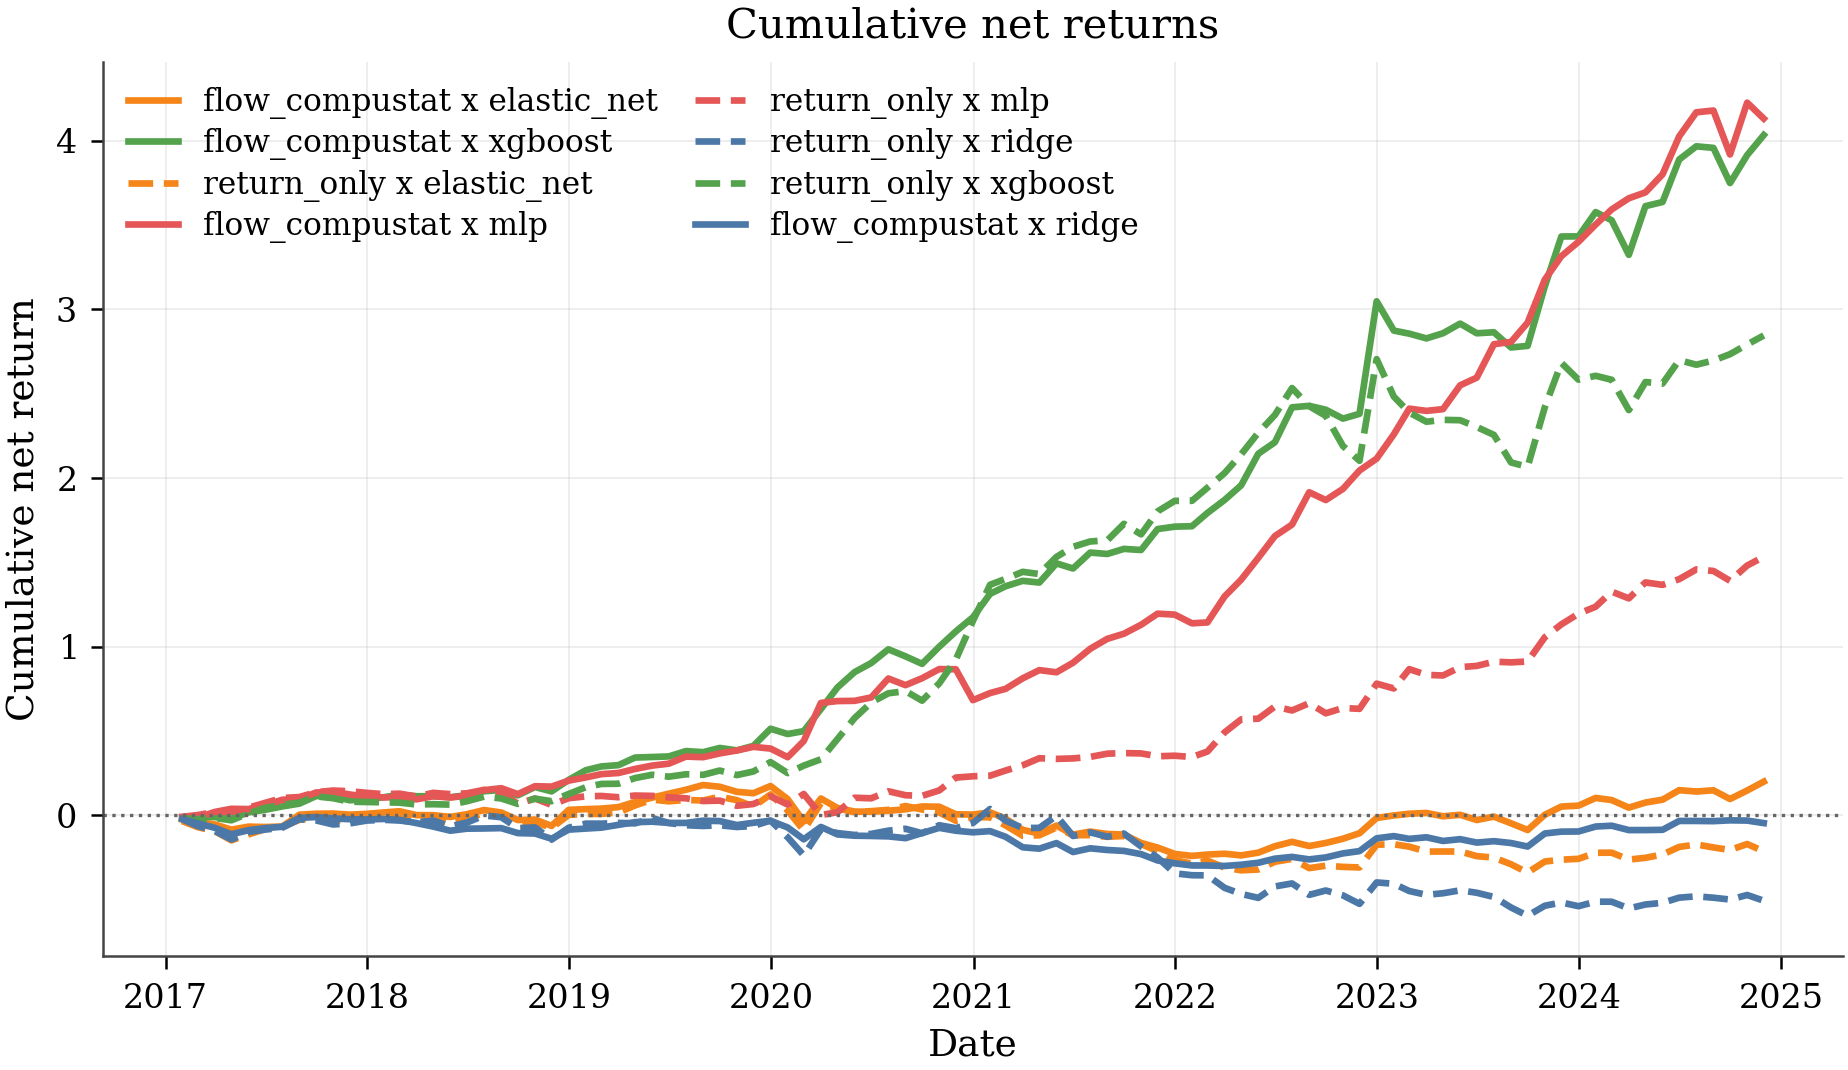
\includegraphics[width=\textwidth]{figures/figure_cumulative_net_returns.png}
\end{minipage}
\hfill
\begin{minipage}[t]{0.49\textwidth}
\centering
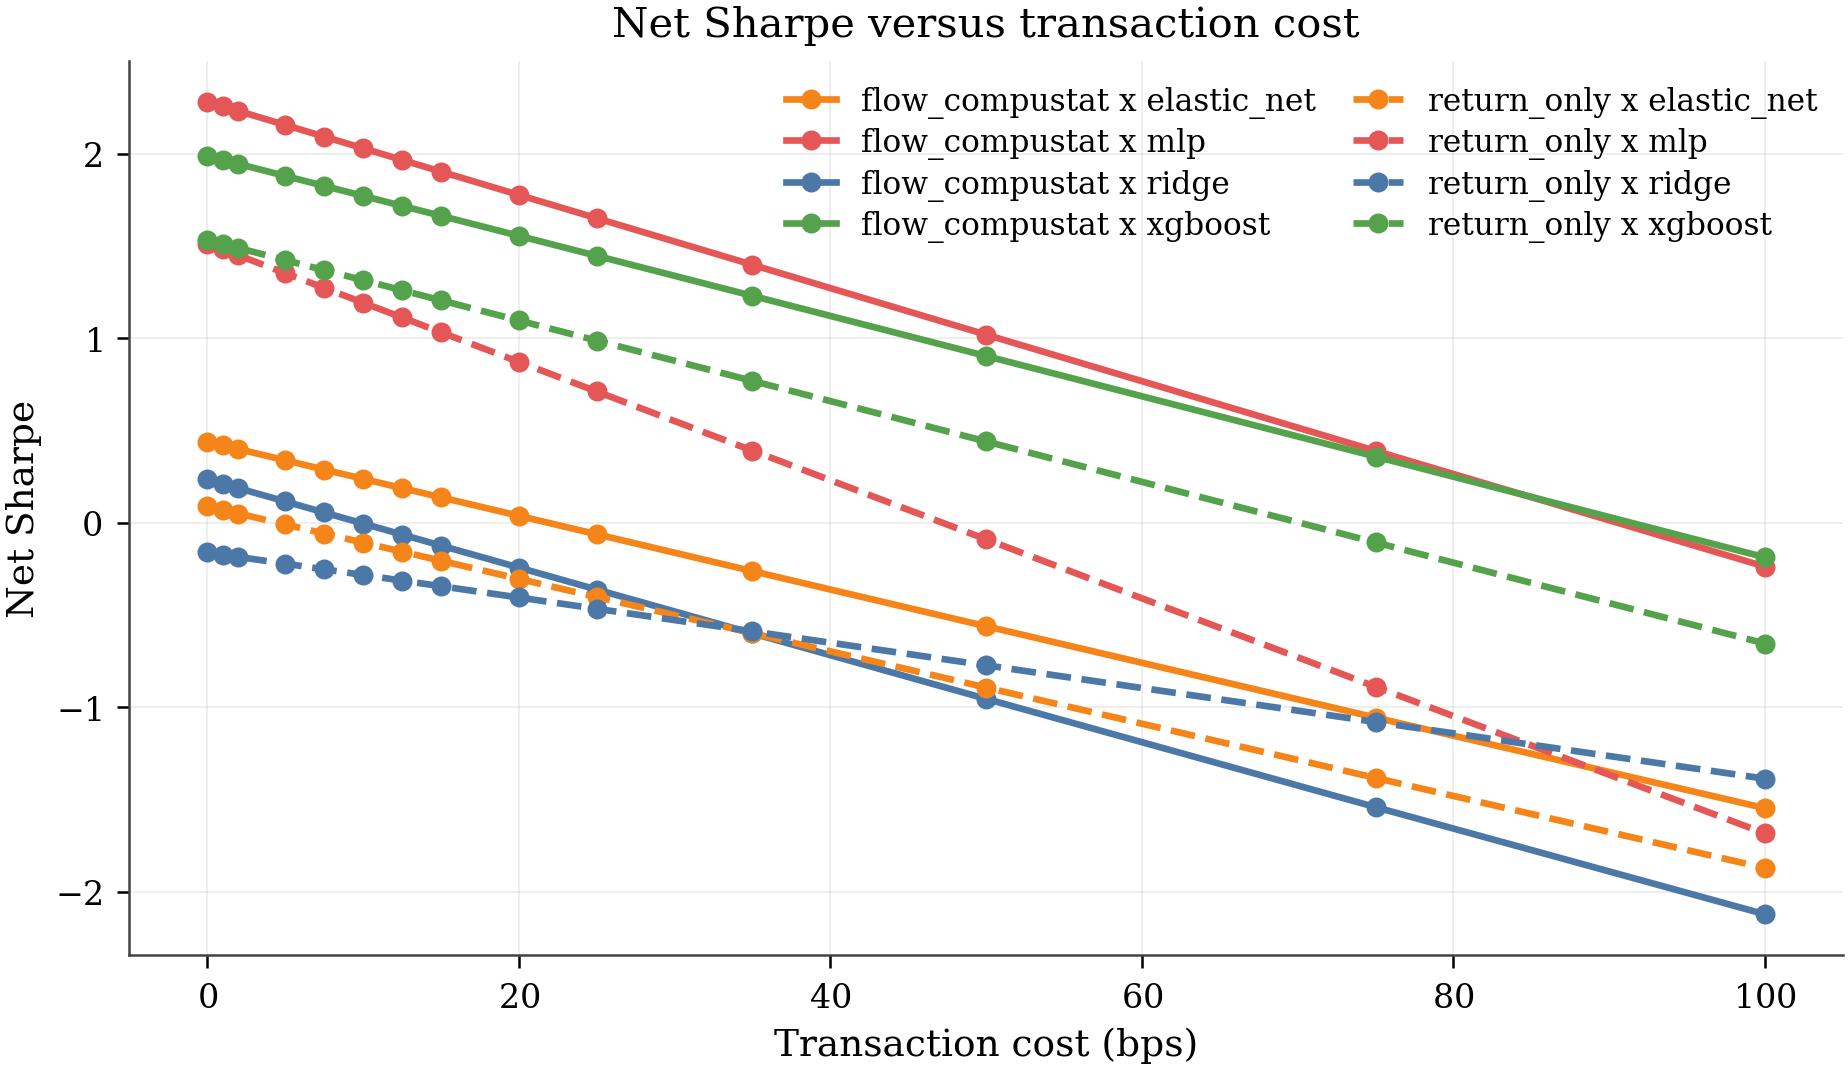
\includegraphics[width=\textwidth]{figures/figure_net_sharpe_vs_cost.png}
\end{minipage}
\caption{Cumulative net performance and transaction-cost sensitivity.
The left panel shows that the leading nonlinear specifications accumulate
economic gains through the final test window. The right panel shows that the
main flow-Compustat models remain positive under materially higher flat costs
than the weaker alternatives. \source{cumulative-return and
cost-sensitivity figures in \code{report/figures/}; cost values align with
\code{table\_cost\_breakeven.csv}}}
\label{fig:main-results}
\end{figure*}

Figure~\ref{fig:main-results} makes the same point visually. The cumulative
return panel shows a clear separation between the leading flow-Compustat
models and the rest of the field. The cost panel shows that the main economic
claim is not driven by an unrealistically low 10 bps assumption. Flat-cost
robustness is not the same as implementation proof, but it is enough to rule
out fragile paper alpha.

\section{Robustness and Ablations}

Table~\ref{tab:classical-tests} sharpens the interpretation of the classical
benchmark comparison. Reversal and z-score reversal are weak under the same
walk-forward protocol. Momentum is stronger and should be treated as the real
classical hurdle. The Newey-West mean-difference tests support exactly that
reading: both leading ML strategies strongly outperform reversal, while the
economic edge over momentum is not statistically decisive in this sample.
Same-protocol classical baselines close the main benchmark gap, and momentum
is a stronger classical benchmark than reversal.

\begin{table*}[t]
\centering
\scriptsize
\setlength{\tabcolsep}{4.5pt}
\begin{tabular*}{\textwidth}{@{\extracolsep{\fill}} lrrrrr@{}}
\toprule
Panel A: same-protocol classical baselines & Net SR & Net ann. & Turnover & Breakeven & Rank-IC $t$ \\
\midrule
Momentum & 0.636 & 15.0\% & 0.92 & 145.6 & 3.34 \\
Reversal plus momentum & 0.491 & 8.2\% & 2.40 & 38.6 & 2.74 \\
Reversal & 0.062 & 1.4\% & 3.13 & 13.9 & -0.12 \\
Z-score reversal & 0.062 & 1.4\% & 3.13 & 13.9 & -0.12 \\
\midrule
\multicolumn{6}{@{}l@{}}{Panel B: selected mean-difference tests versus classical baselines} \\
\midrule
Comparison & Months & Monthly diff. & Annualized diff. & NW $t$ & Interpretation \\
\midrule
Flow-Compustat MLP $-$ reversal & 95 & 1.66\% & 19.93\% & 3.34 & Strong outperformance \\
Flow-Compustat XGBoost $-$ reversal & 95 & 1.65\% & 19.82\% & 4.28 & Strong outperformance \\
Flow-Compustat MLP $-$ z-score reversal & 95 & 1.66\% & 19.93\% & 3.34 & Strong outperformance \\
Flow-Compustat XGBoost $-$ z-score reversal & 95 & 1.65\% & 19.82\% & 4.28 & Strong outperformance \\
Flow-Compustat MLP $-$ momentum & 95 & 0.53\% & 6.35\% & 0.74 & Economic, not decisive \\
Flow-Compustat XGBoost $-$ momentum & 95 & 0.52\% & 6.25\% & 0.56 & Economic, not decisive \\
\bottomrule
\end{tabular*}
\caption{Classical benchmark levels and same-protocol model-difference tests.
\source{same-protocol classical baseline and model-difference CSVs in
\code{report/tables/}}}
\label{tab:classical-tests}
\end{table*}

The other robustness dimensions are also informative. Table~\ref{tab:implementation}
summarizes the key implementation and exposure diagnostics. Rebalancing
results from \code{table\_rebalance\_robustness.csv} show that quarterly
trading cuts average turnover from roughly 2.2 to 0.86 for the leading
flow-Compustat models, but monthly rebalancing still produces the stronger net
Sharpe. Alpha and beta estimates from \code{table\_alpha\_beta.csv} show that
the main MLP and XGBoost strategies earn positive net monthly alpha of about
1.98\% and 1.89\%, respectively, with low or negative market beta. These
results are consistent with a cross-sectional stock-selection effect rather
than a disguised market bet.

\begin{table*}[t]
\centering
\scriptsize
\setlength{\tabcolsep}{4.5pt}
\begin{tabular*}{\textwidth}{@{\extracolsep{\fill}} lrrr@{}}
\toprule
Panel A: incremental-value tests & Monthly diff. & Annualized diff. & NW $t$ \\
\midrule
Flow-Compustat MLP $-$ Return-only MLP & 0.75\% & 9.05\% & 2.53 \\
Flow-Compustat XGBoost $-$ Return-only XGBoost & 0.27\% & 3.24\% & 0.90 \\
Flow-Compustat MLP $-$ Flow-Compustat XGBoost & 0.01\% & 0.10\% & 0.03 \\
\midrule
\multicolumn{4}{@{}l@{}}{Panel B: implementation and exposure diagnostics} \\
\midrule
Strategy & Monthly / quarterly net SR & Monthly / quarterly turnover & Net alpha / beta \\
\midrule
Flow-Compustat MLP & 2.03 / 1.85 & 2.21 / 0.86 & 1.98\% / -0.17 \\
Flow-Compustat XGBoost & 1.77 / 1.37 & 2.18 / 0.86 & 1.89\% / -0.10 \\
\bottomrule
\end{tabular*}
\caption{Selected incremental-value, implementation, and exposure diagnostics.
\source{\code{table\_model\_incremental\_tests.csv},
\code{table\_rebalance\_robustness.csv}, and
\code{table\_alpha\_beta.csv} in \code{report/tables/}}}
\label{tab:implementation}
\end{table*}

Prediction sorting also looks economically credible. Figure~\ref{fig:robust}
shows clear separation between the tails of the forecast distribution. The
flow-Compustat MLP delivers a gross top-minus-bottom spread of about 2.00\%
per month, with decile 1 averaging $-1.02\%$ and decile 10 averaging 1.05\%.
The flow-Compustat XGBoost model is similar, at roughly 1.99\% per month.
Monotonicity is strongest at the tails rather than perfectly smooth in every
intermediate decile, which is typical for noisy cross-sectional return data.

\begin{figure*}[t]
\centering
\begin{minipage}[t]{0.49\textwidth}
\centering
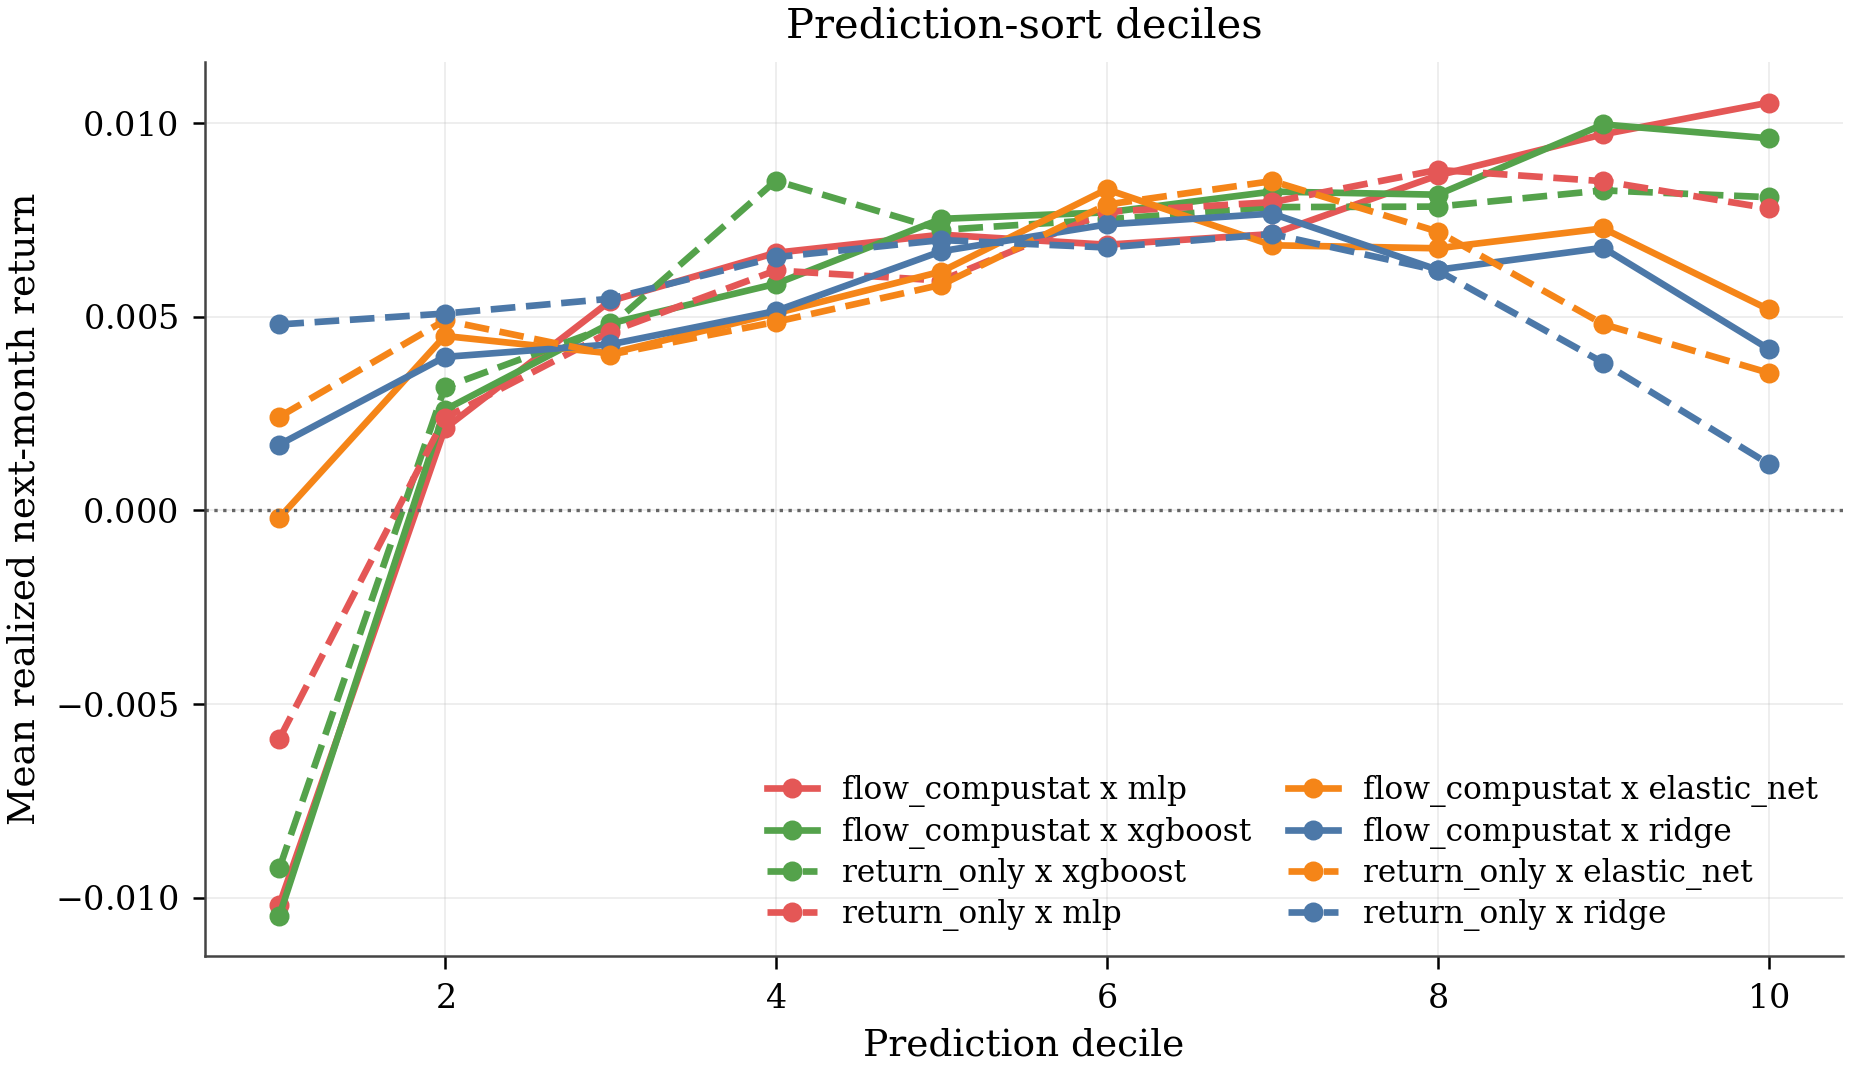
\includegraphics[width=\textwidth]{figures/figure_prediction_deciles.png}
\end{minipage}
\hfill
\begin{minipage}[t]{0.49\textwidth}
\centering
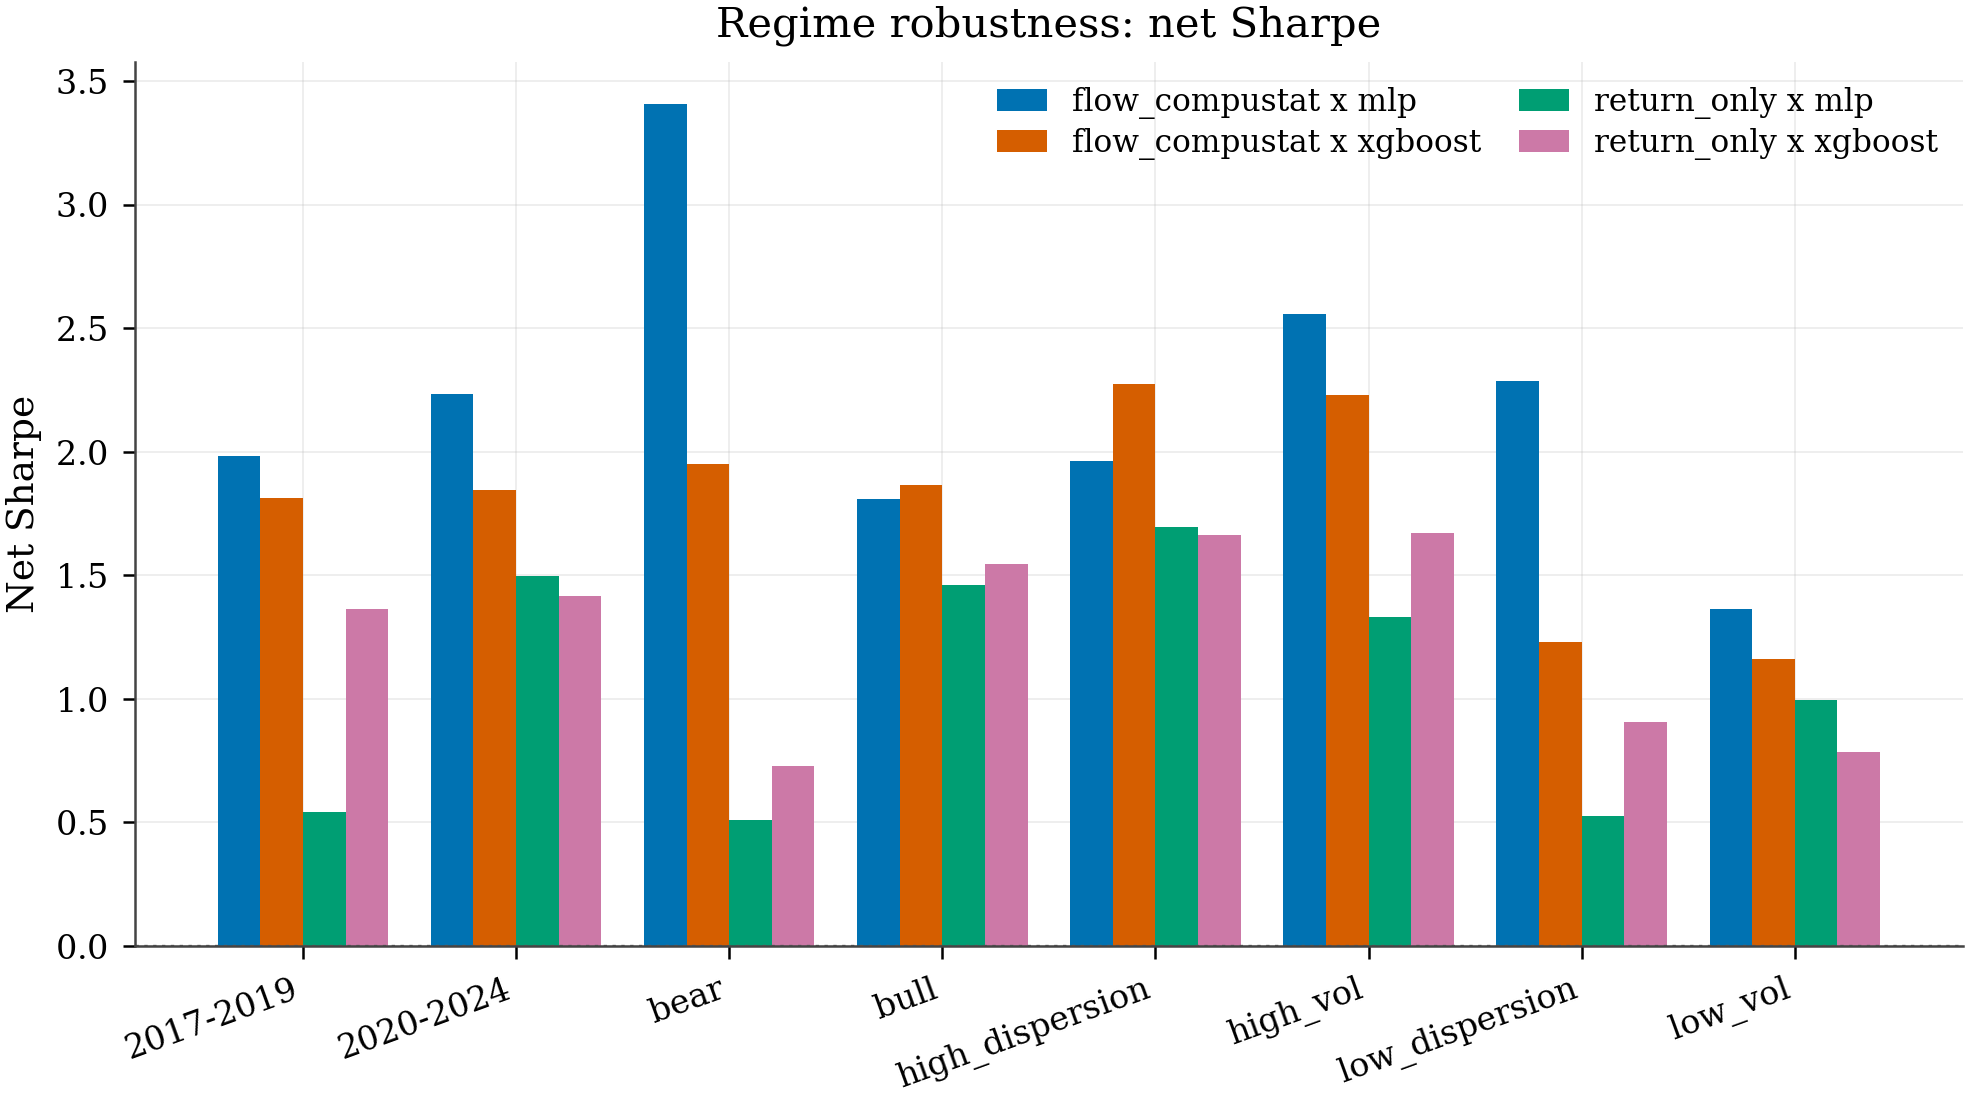
\includegraphics[width=\textwidth]{figures/figure_regime_net_sharpe.png}
\end{minipage}
\caption{Prediction-decile evidence and regime-conditional net Sharpe.
The left panel shows that the best models sort the tails well. The right panel
shows that performance varies materially across market states, with the
strongest outcomes in bear and high-volatility regimes. \source{\code{figure\_prediction\_deciles.png}
and \code{figure\_regime\_net\_sharpe.png} in \code{report/figures/};
supporting values align with the prediction-decile and regime-robustness CSVs
in \code{report/tables/}}}
\label{fig:robust}
\end{figure*}

Regime dependence is present in performance even when it does not help as an
explicit feature input. According to
\code{table\_regime\_robustness.csv}, the flow-Compustat MLP reaches
net Sharpe 3.41 in bear months and 2.56 in high-volatility months, while still
remaining positive in bull and low-volatility states. The corresponding
XGBoost model reaches 1.95 in bear months and 2.23 in high-volatility months.
This supports the interpretation that mean reversion is conditional and
state-dependent.

Subperiod robustness points in the same direction. Table~\ref{tab:regime-summary}
summarizes the regime and subperiod net Sharpe evidence for the two leading
models. The flow-Compustat MLP posts net Sharpe 1.98 in 2017-2019 and 2.23 in
2020-2024, while the corresponding XGBoost specification delivers 1.81 and
1.84. High-dispersion months are especially favorable for XGBoost, at net
Sharpe 2.27, whereas low-dispersion and low-volatility states remain positive
but weaker for both leading models. The signal is therefore not a one-episode
artifact, but it is stronger when cross-sectional opportunities widen.

\begin{table*}[t]
\centering
\scriptsize
\setlength{\tabcolsep}{4.5pt}
\begin{tabular*}{\textwidth}{@{\extracolsep{\fill}} lrr@{}}
\toprule
Regime or subperiod & Flow-Compustat MLP net SR & Flow-Compustat XGBoost net SR \\
\midrule
2017-2019 & 1.981 & 1.813 \\
2020-2024 & 2.232 & 1.843 \\
Bear market months & 3.408 & 1.952 \\
Bull market months & 1.808 & 1.863 \\
High-volatility months & 2.559 & 2.229 \\
Low-volatility months & 1.361 & 1.161 \\
High-dispersion months & 1.962 & 2.273 \\
Low-dispersion months & 2.286 & 1.229 \\
\bottomrule
\end{tabular*}
\caption{Selected regime-conditional and subperiod net Sharpe results for the
two leading strategies.
\source{\code{table\_regime\_robustness.csv} in \code{report/tables/}}}
\label{tab:regime-summary}
\end{table*}

However, the direct regime-feature ablation is not supportive for the best
models. Table~\ref{tab:supplementary} shows that adding a small lagged regime
block to the flow-Compustat models lowers net Sharpe from 2.028 to 1.520 for
the MLP and from 1.770 to 1.439 for XGBoost. The return-only MLP improves
modestly when regime features are added, but that gain is not enough to
challenge the main model. The right interpretation is that regime
dependence matters for evaluation, but simple regime features are not a robust
incremental input to the strongest specification. We therefore treat regime
dependence mainly as an evaluation dimension.

\begin{table*}[t]
\centering
\scriptsize
\setlength{\tabcolsep}{3pt}
\begin{tabular*}{\textwidth}{@{\extracolsep{\fill}} lrrrrr@{}}
\toprule
Panel A: supplementary target and seed checks & Net SR & Breakeven & Rank-IC $t$ & Mean seed SR & Seed std. \\
\midrule
Flow-Compustat MLP on excess-return target & 2.970 & 124.0 & 4.51 & -- & -- \\
Flow-Compustat MLP multi-seed stability & -- & -- & -- & 1.968 & 0.227 \\
\midrule
\multicolumn{6}{@{}l@{}}{Panel B: direct regime-feature ablation at 10 bps} \\
\midrule
Specification & Net SR & Reference SR & Delta SR & Target & Interpretation \\
\midrule
Flow-Compustat-regime $\times$ MLP & 1.520 & 2.028 & -0.508 & Raw return & Weaker than main model \\
Flow-Compustat-regime $\times$ XGBoost & 1.439 & 1.770 & -0.332 & Raw return & Weaker than flow-Compustat XGBoost \\
Return-regime $\times$ MLP & 1.398 & 1.192 & 0.207 & Raw return & Modest help to return-only MLP \\
Return-regime $\times$ XGBoost & 1.267 & 1.313 & -0.046 & Raw return & Roughly flat to weaker \\
\bottomrule
\end{tabular*}
\caption{Supplementary robustness checks and direct regime-feature ablations.
These results support, but do not replace, the final audited raw-return
walk-forward result. \source{\code{table\_supplementary\_robustness.csv}
in \code{report/tables/}}}
\label{tab:supplementary}
\end{table*}

The remaining supplementary results are favorable. Re-estimating the main
flow-Compustat MLP on the excess-return target yields net Sharpe 2.97 and
breakeven costs near 124 bps. A three-seed MLP robustness check gives mean net
Sharpe 1.97 with standard deviation 0.23, minimum 1.72, and maximum 2.16.
These results reinforce the baseline finding, but they should remain
supplementary because the headline result is the final audited raw-return
walk-forward result.

These checks help bound the interpretation of the main result. The
excess-target exercise shows that the signal is not simply a proxy for market
direction, and the multi-seed exercise shows that the main MLP is not a
single favorable initialization. At the same time, neither robustness layer
changes the hierarchy of evidence: the paper's primary claim continues to rest
on the raw-return final audited walk-forward package because that is the
protocol used for the final comparison set. These checks do not
replace the main raw-target final audited result.

\section{Limitations}

The main limitation is implementation realism. The report uses a shared
flat-bps transaction-cost model and the provided Monthly CRSP universe, but it
cannot apply true price, share-code, exchange, microcap, or liquidity screens
because the required fields are absent from the provided extract. That means
the paper demonstrates robust academic signal quality under a controlled
backtest rather than a fully executable production strategy.

The second limitation is that monthly data compresses trading frictions into a
single turnover penalty. There is no explicit market-impact model, no
order-book information, and no richer execution schedule. Likewise, delisting
return handling is limited to what is already present in the provided source
data. These constraints are acceptable within the assignment but should narrow
the strength of any external investment claim.

A related limitation is that the regime block is deliberately simple. The
report uses lagged market-return, volatility, drawdown, and dispersion proxies
rather than a full macro state model. That is appropriate for a disciplined
course project, but it means the regime results should be read as evidence of
conditional heterogeneity rather than as a complete map from macro states to
expected reversal profits.

The final limitation is conceptual. Even with strictly out-of-sample
evaluation, ML finance results remain exposed to model-selection risk and
multiple-testing risk. The protocol protects the 2017-2024 test folds from
direct leakage, but
it does not make the broader research process immune to data-mining concerns.
For that reason, the report's strongest claim is comparative and conditional:
within the provided-data environment, nonlinear models with audited
flow-Compustat inputs rank stocks better than the natural reversal
benchmarks.

\section{Conclusion}

The final evidence supports a clear but measured conclusion. Conditional
nonlinear models improve cross-sectional mean-reversion forecasting relative to
simple reversal rules, and the improvement survives a common 10 bps cost
assumption. The strongest specification is the flow-Compustat MLP,
with net Sharpe 2.03, annualized net return 21.4\%, breakeven costs near 90
bps, and strong rank-IC evidence. Flow-Compustat XGBoost is the closest
competitor and confirms that the result is not tied to a single nonlinear
architecture.

The conclusion becomes more nuanced once the correct classical benchmark is
used. ML strongly dominates reversal and z-score reversal, but momentum remains
economically relevant and is not cleanly rejected by the same-protocol
mean-difference tests. Regime dependence also matters, but mainly as a source
of performance heterogeneity rather than as an explicit feature block that
improves the strongest model. Overall, the project provides credible
out-of-sample evidence that conditional mean reversion is strongest when
nonlinear methods are combined with firm-level flow characteristics, while also
making clear that the result remains an academic ML-in-finance finding rather
than a complete tradability proof.
